\thispagestyle{main}
\chapter{Latex部分代码示例}
\thispagestyle{main}

\section{图片}

\subsection{单张图片示例}

\par \textbf{注意,图片的标题在下面。}

\begin{figure}[!ht]
    \centering
    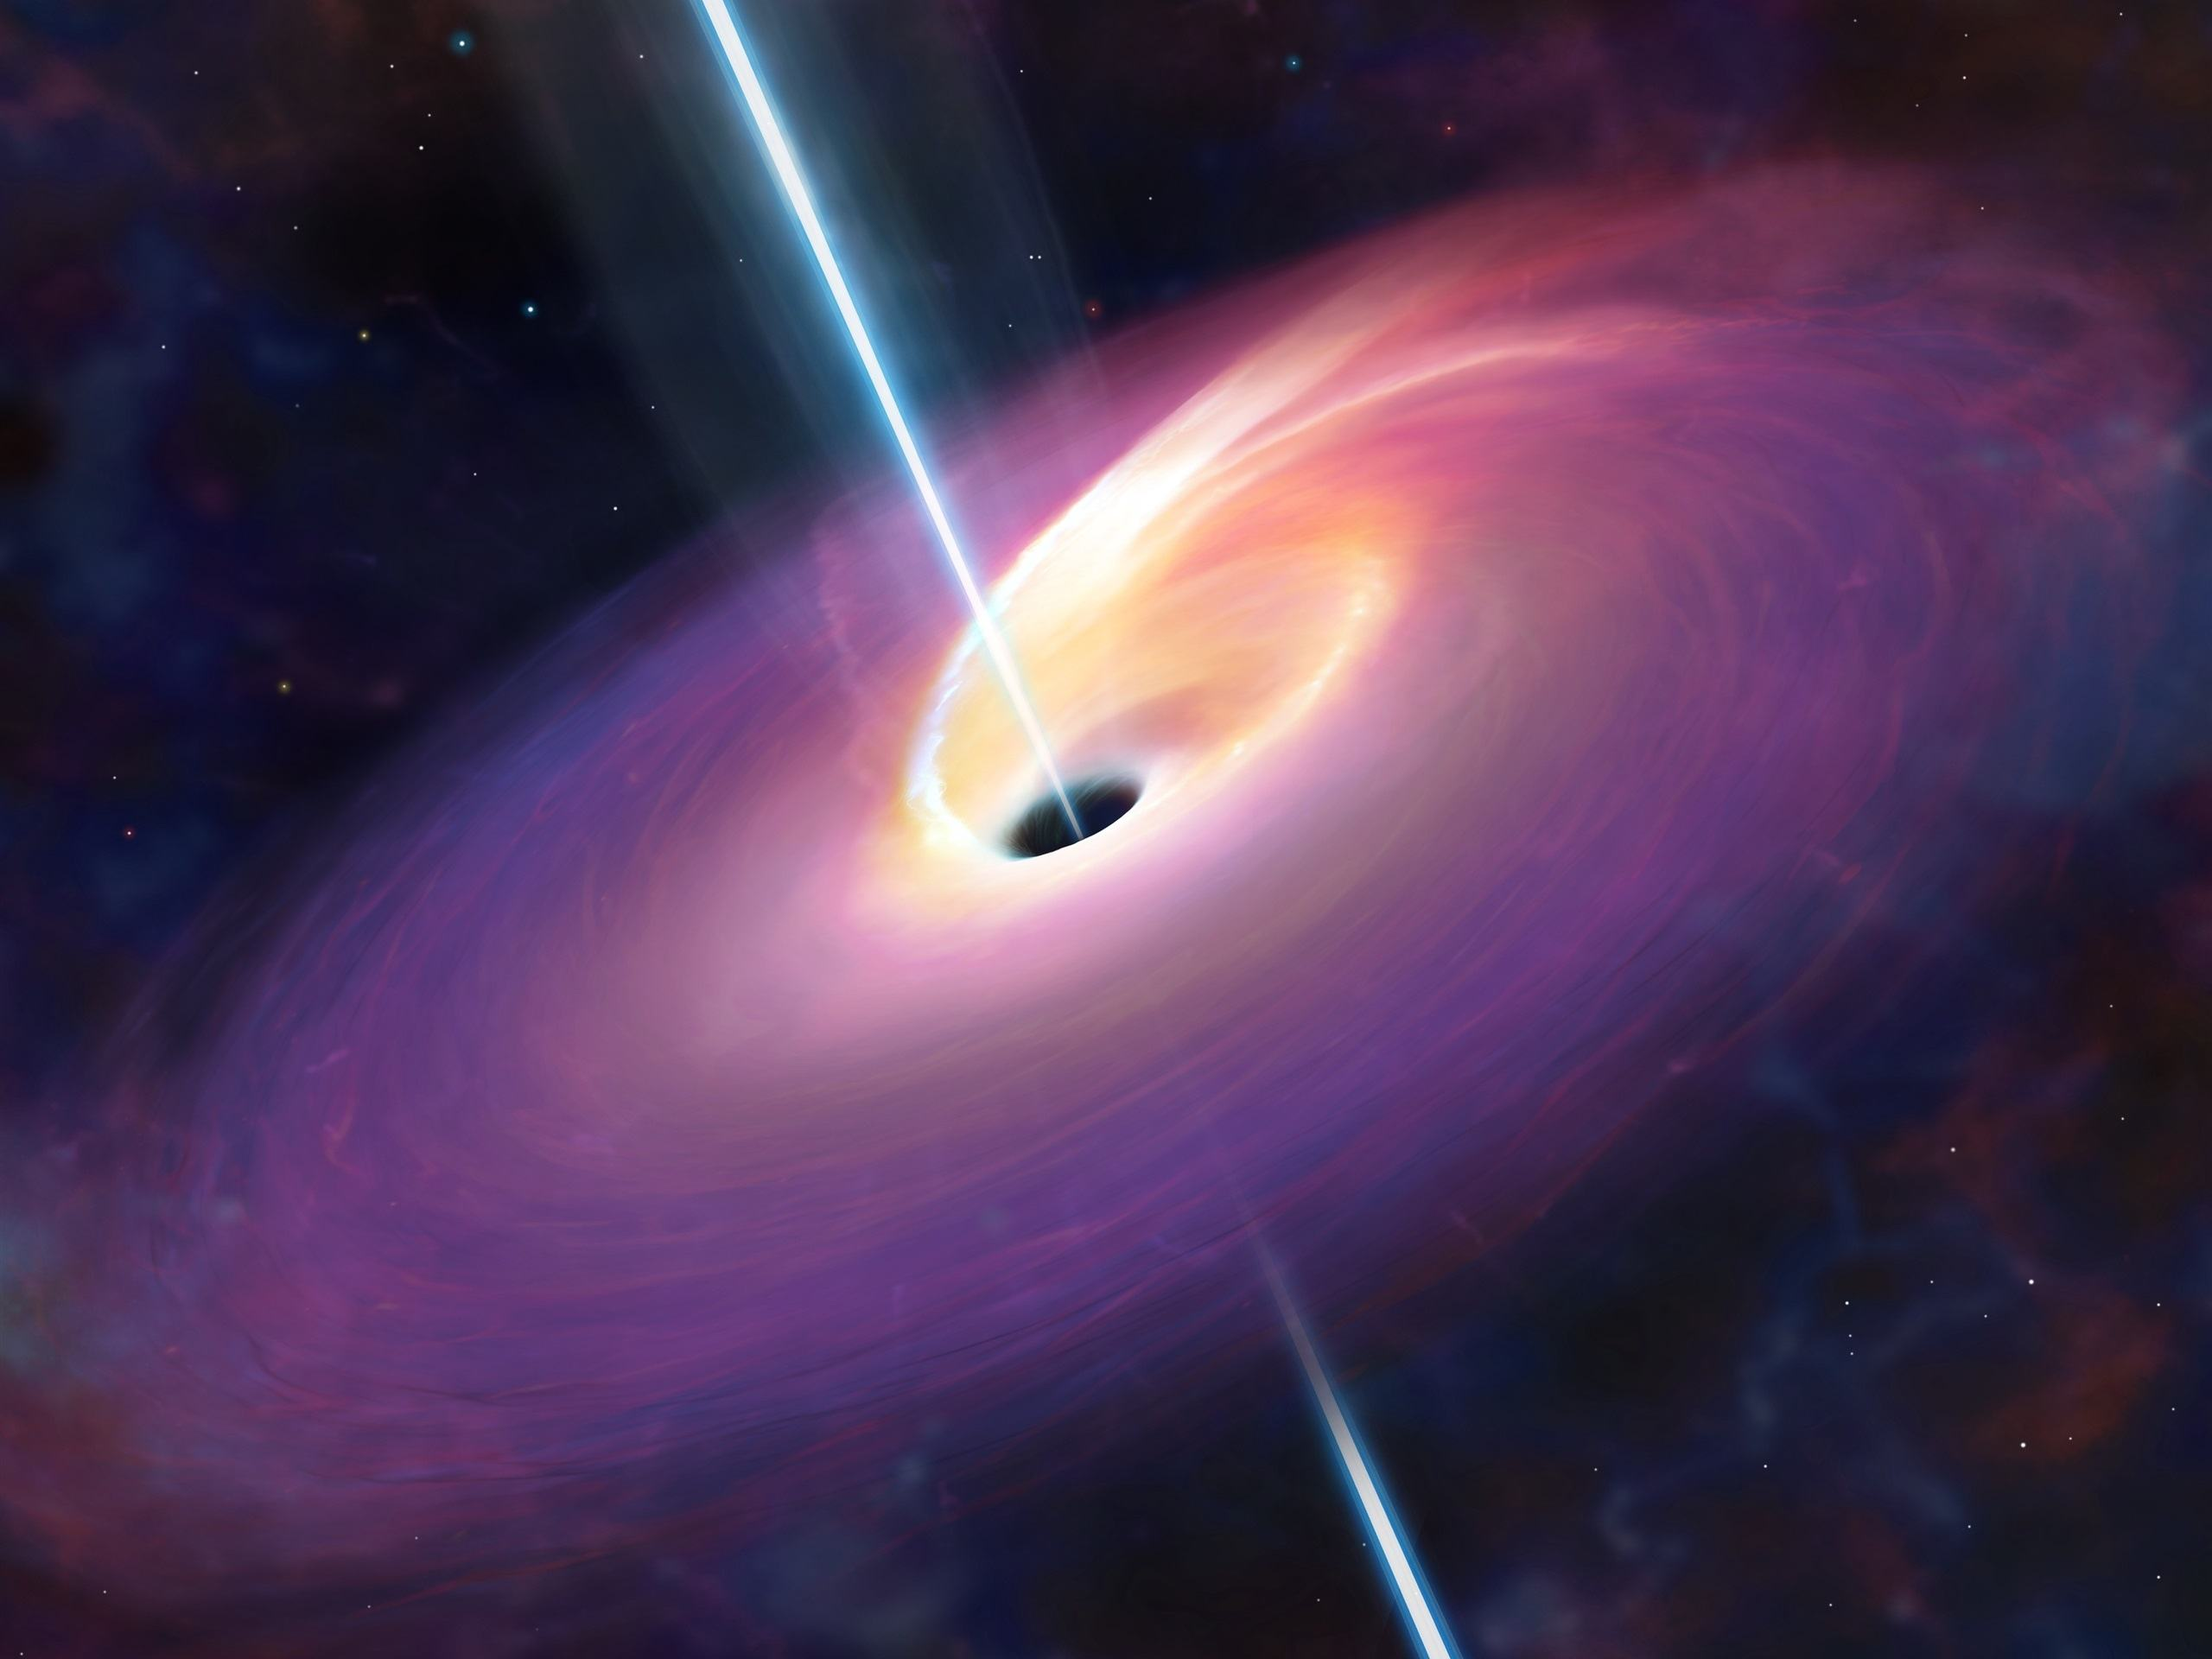
\includegraphics[width=2.5in]{images/blackhole.jpeg}
    \caption{黑洞}
    \label{fig:blackhole1}
\end{figure}
图\ref{fig:blackhole1}是单个黑洞图片。

\subsection{多张图片示例}

\begin{figure*}[!ht]
    \centering
    \subfloat[黑洞1。]{
        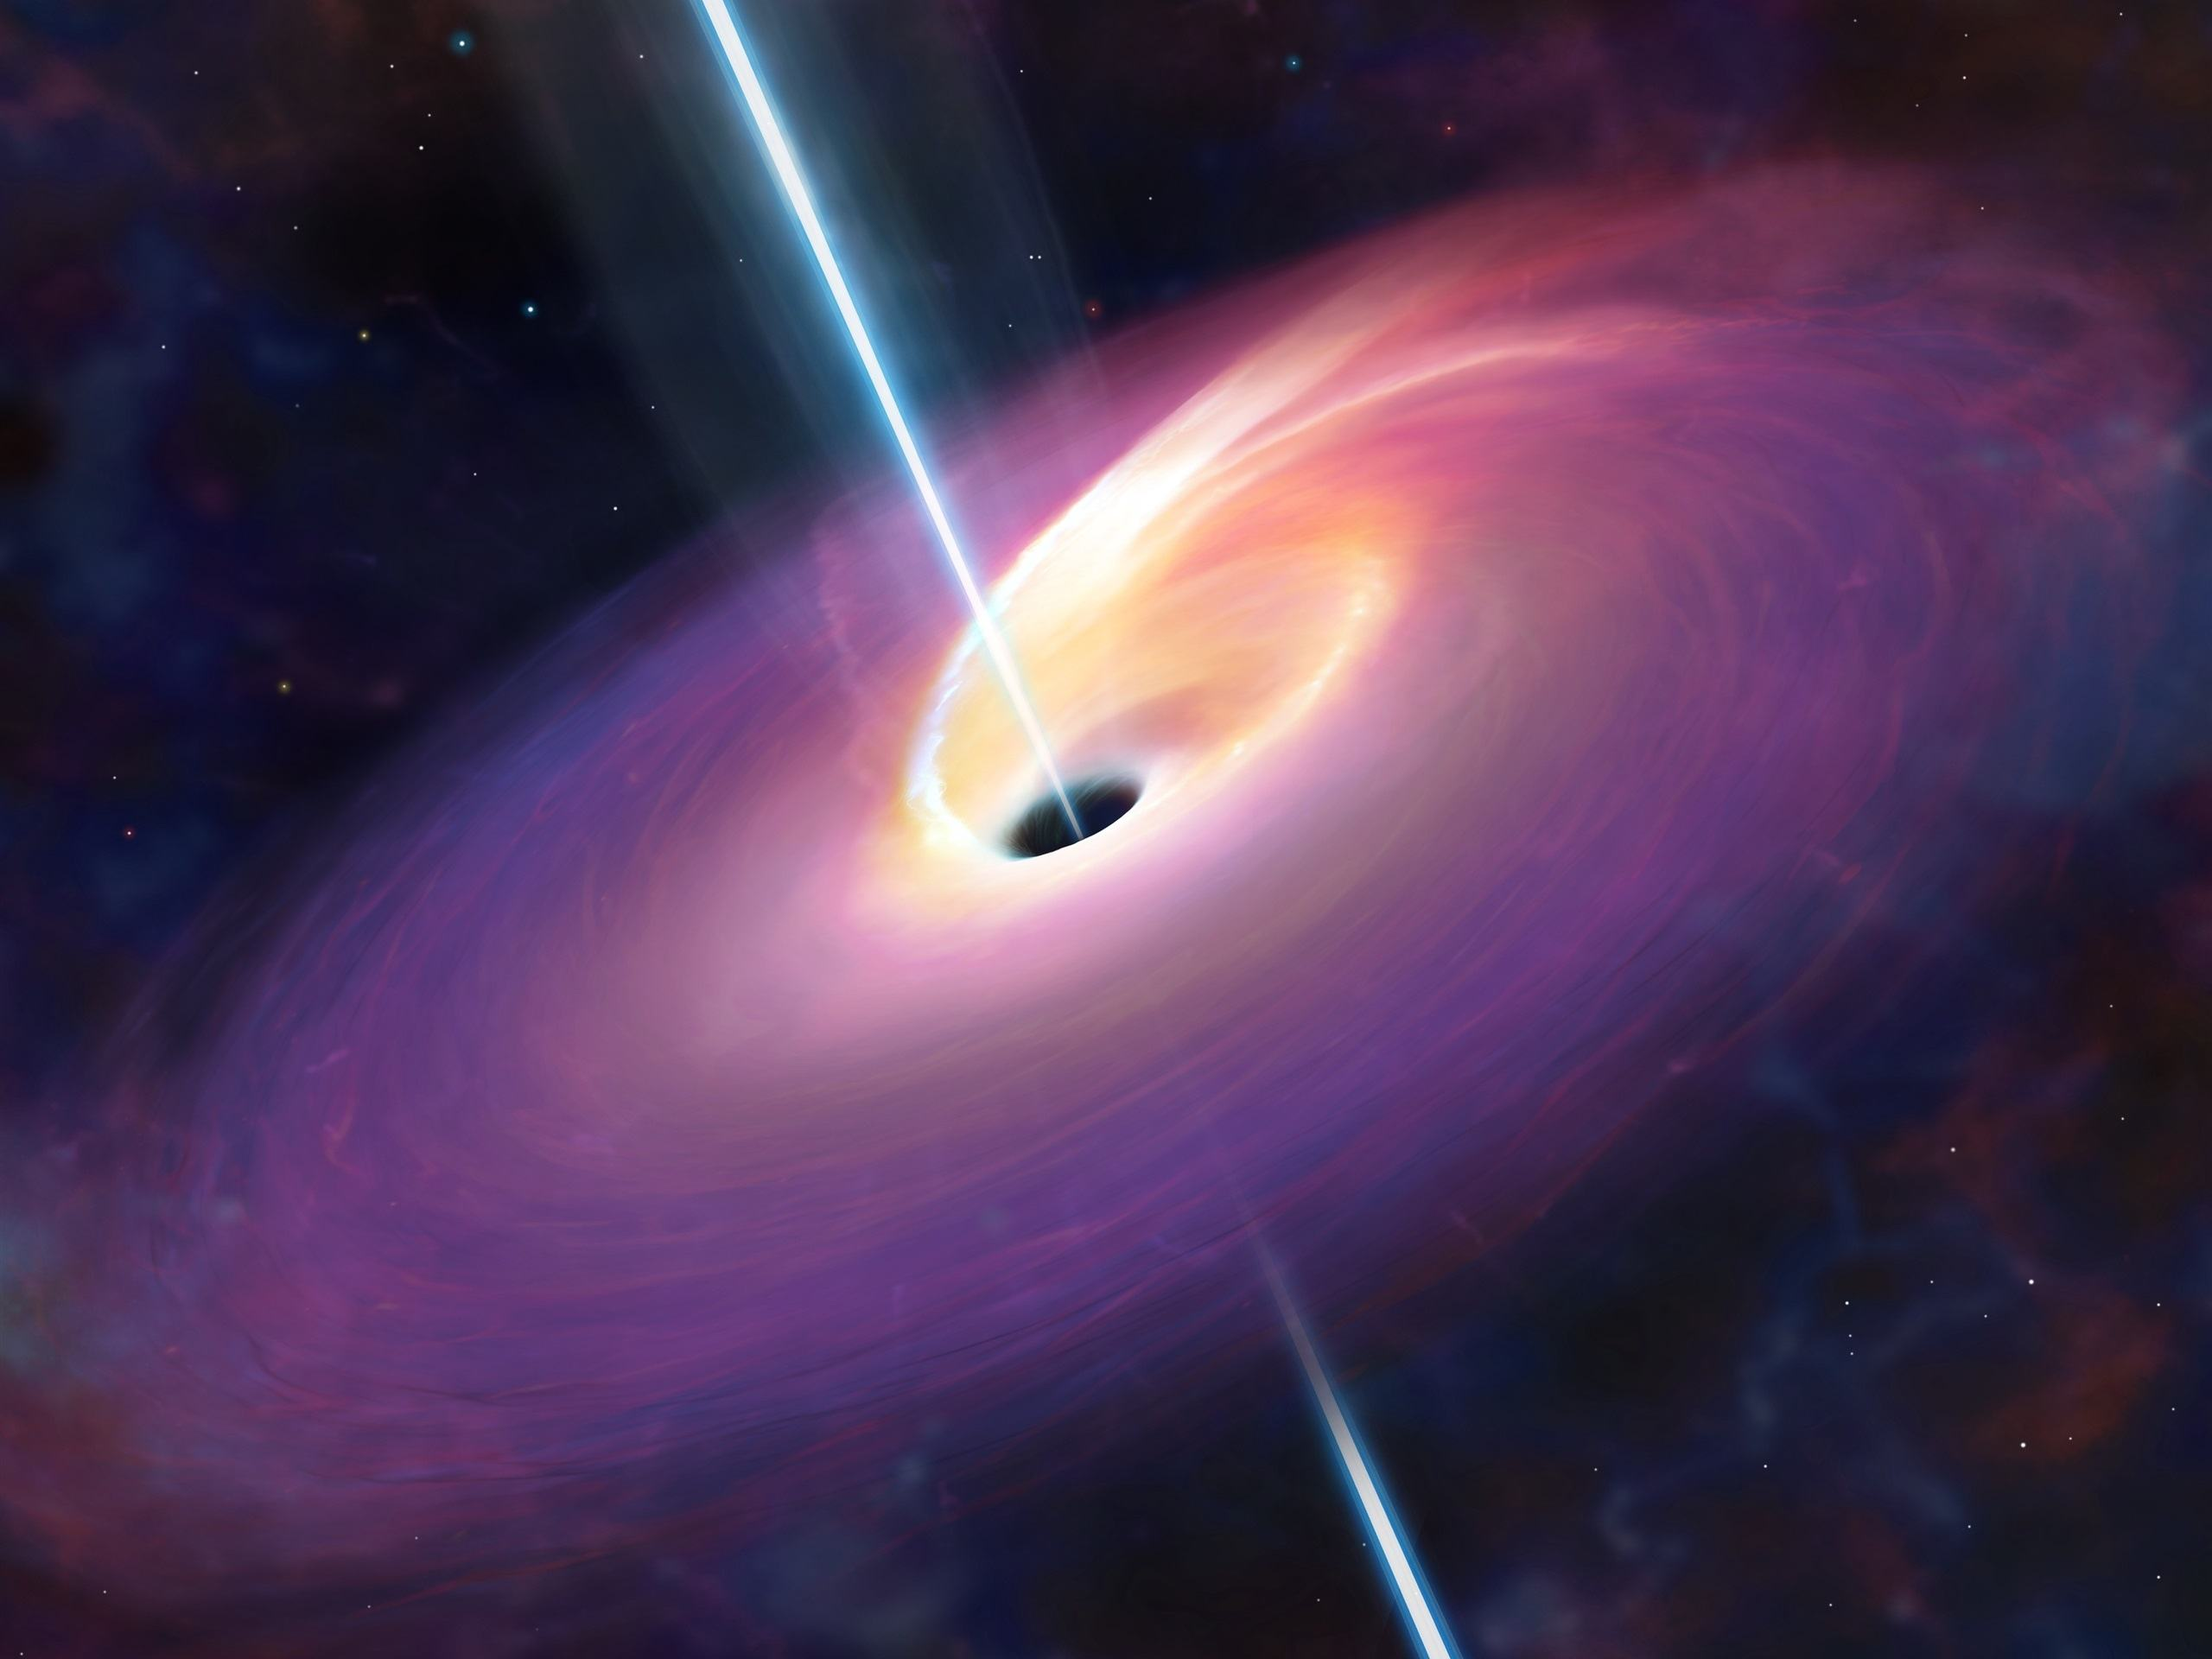
\includegraphics[width = 0.45\textwidth]{images/blackhole.jpeg}
    }
    \hfill
    \subfloat[黑洞2。]{
        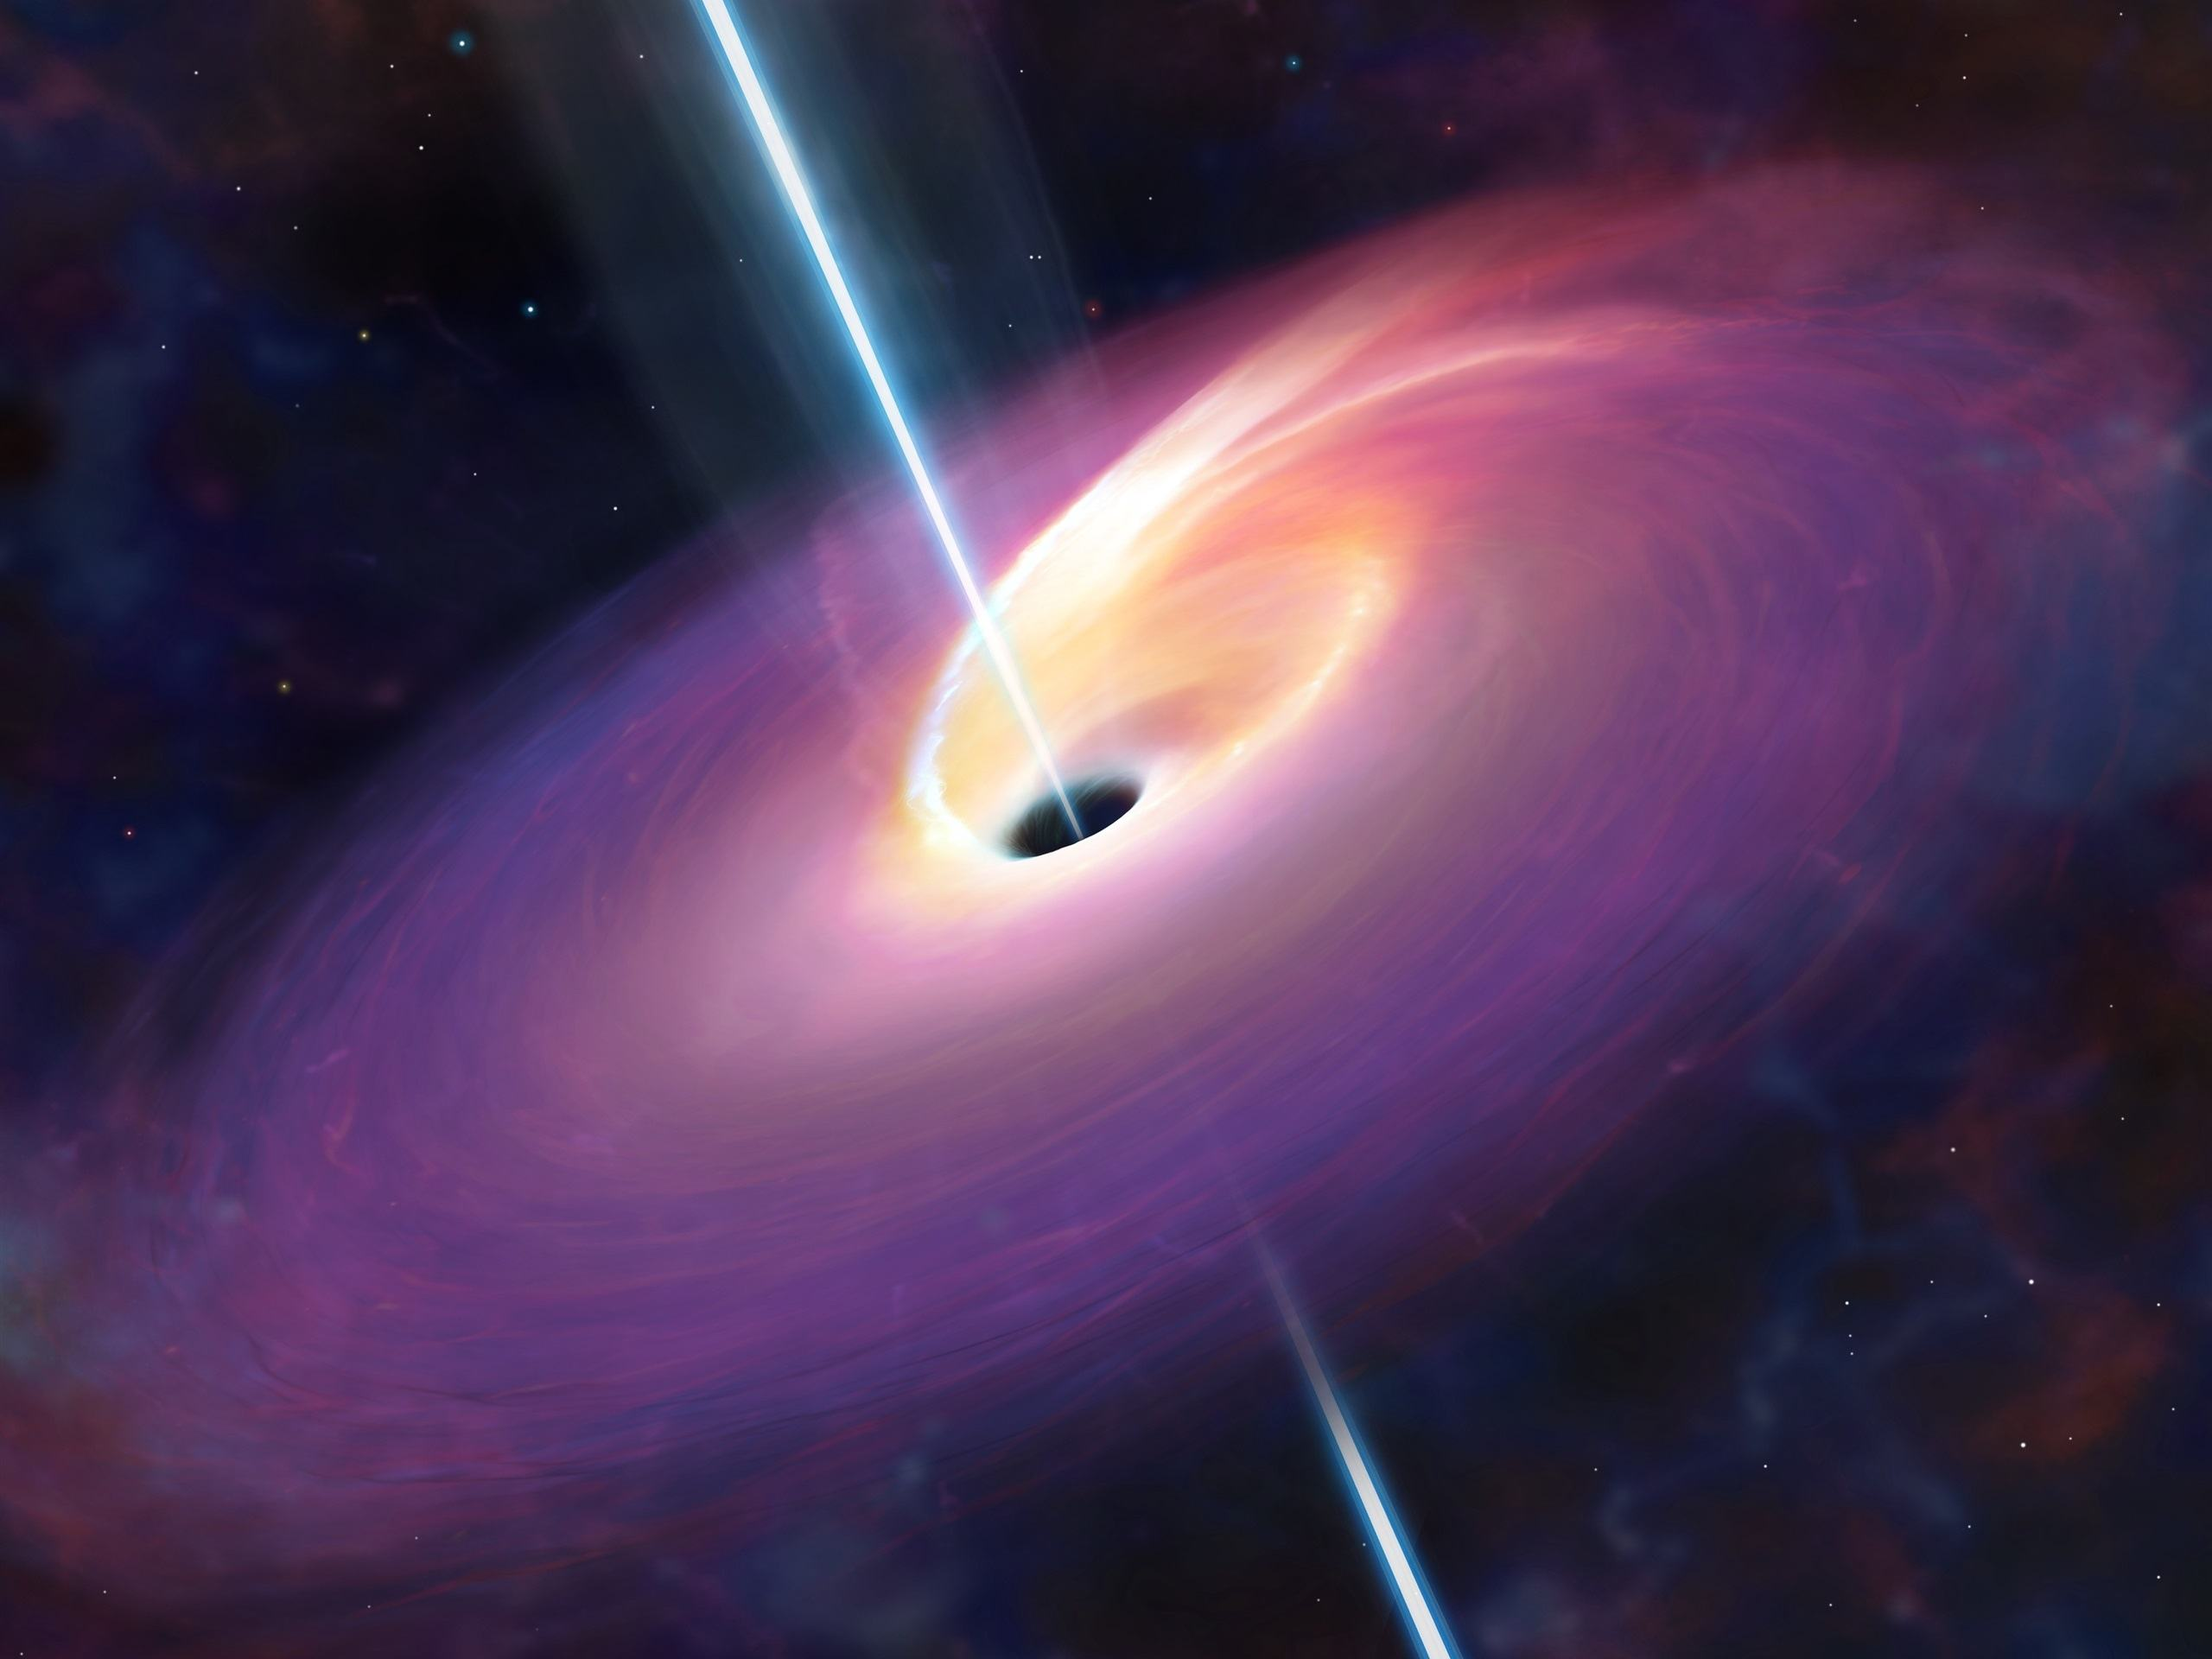
\includegraphics[width = 0.45\textwidth]{images/blackhole.jpeg}
    }
    \\
    \subfloat[黑洞3。]{
        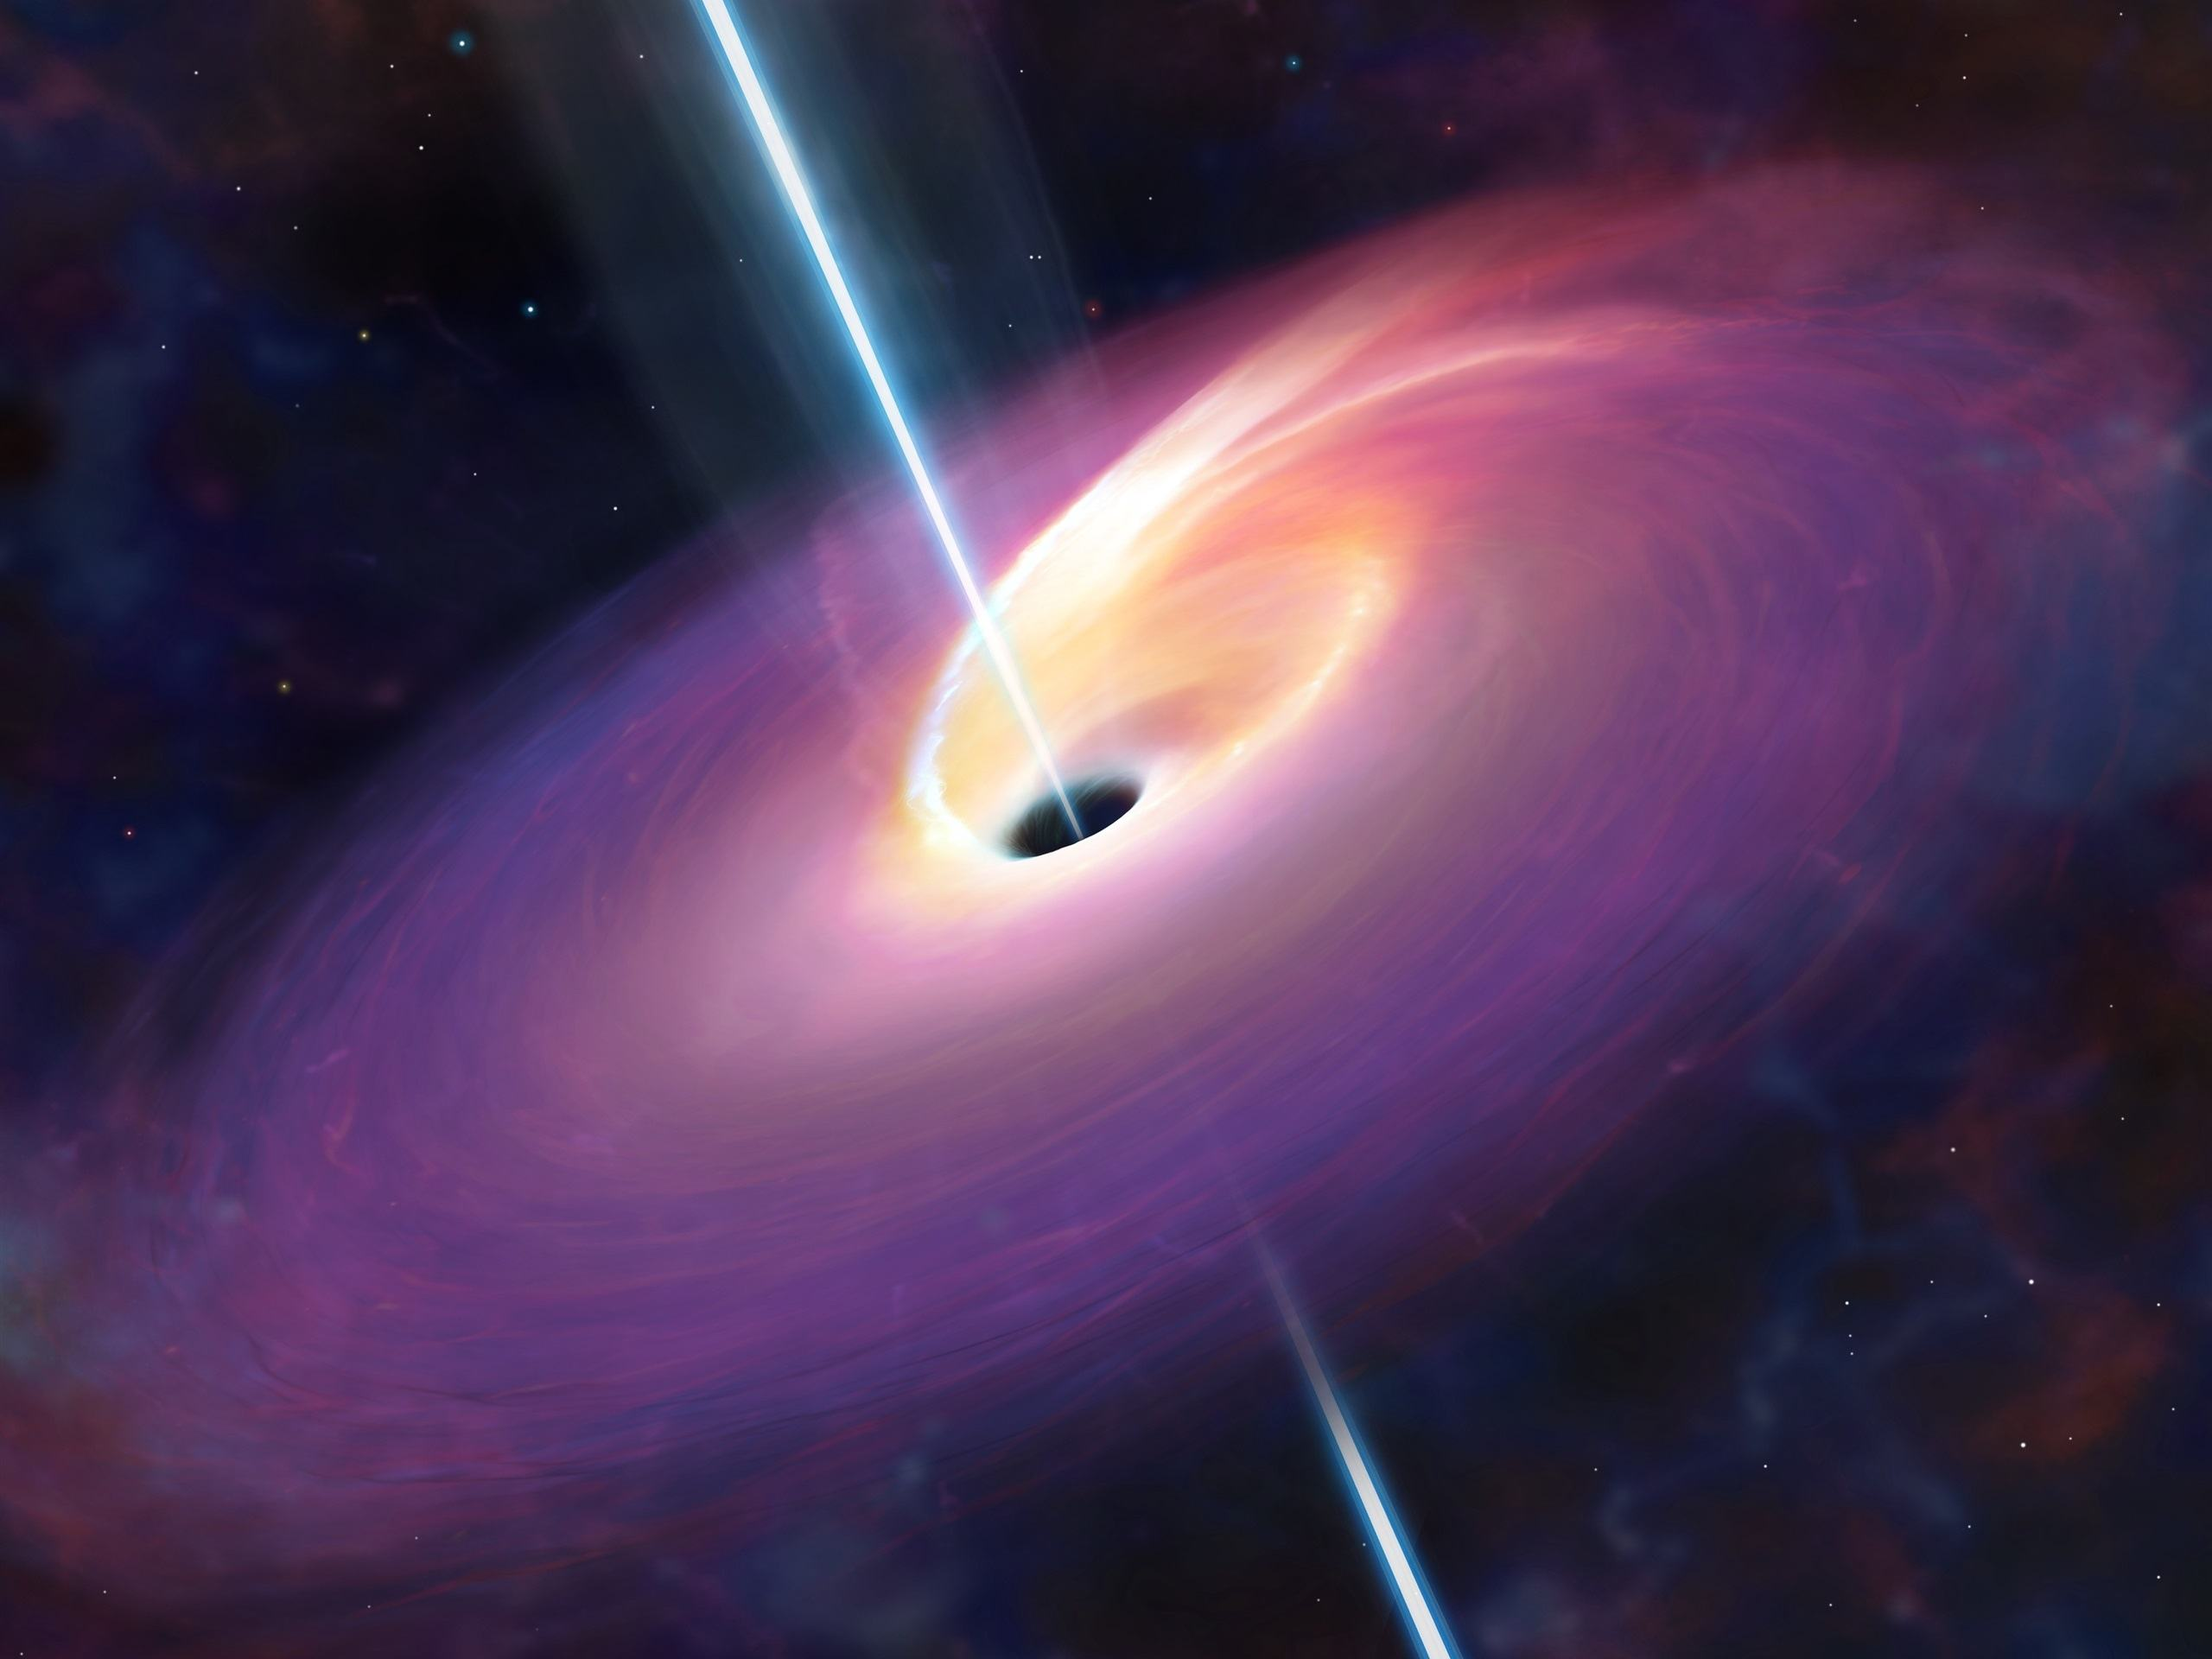
\includegraphics[width = 0.45\textwidth]{images/blackhole.jpeg}
    }
    \hfill
    \subfloat[黑洞4。]{
        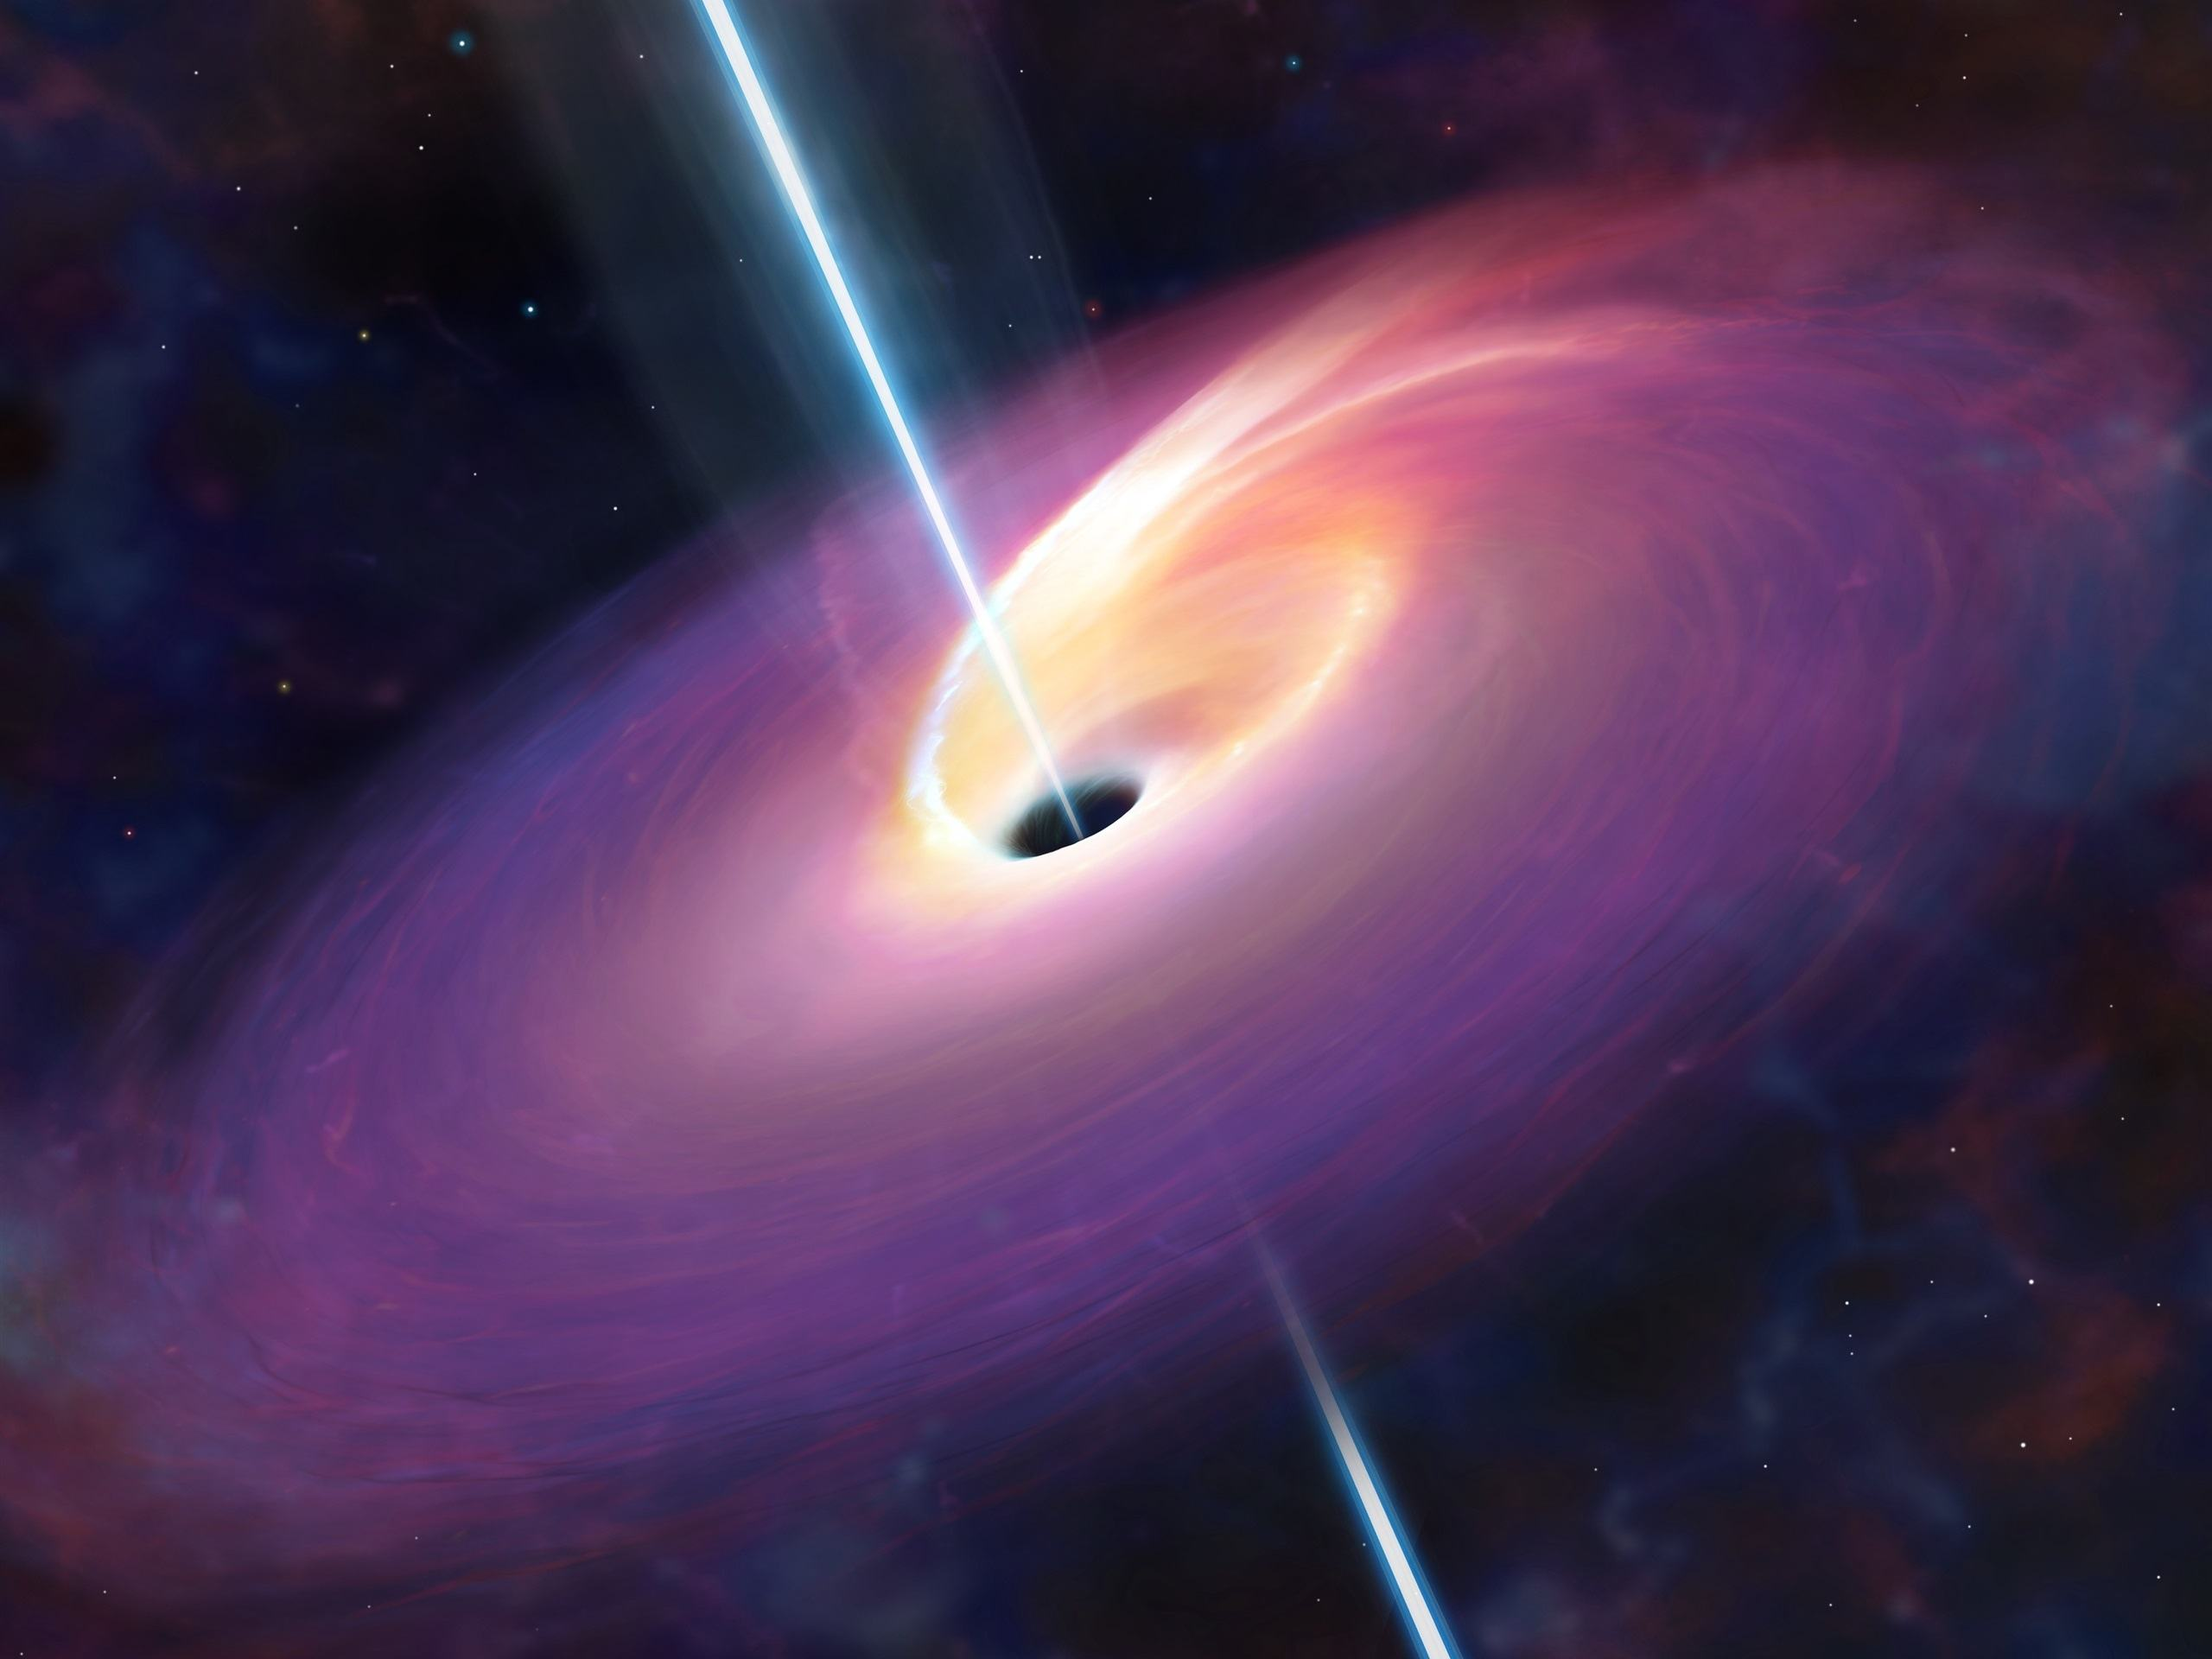
\includegraphics[width = 0.45\textwidth]{images/blackhole.jpeg}
    }
    \caption{多个黑洞}
    \label{fig:blackhole2}
\end{figure*}

图\ref{fig:blackhole2}是多个黑洞图片并列。

\section{表格}

\par \textbf{注意,表格的标题在上面。}

\begin{table}[!ht]
\centering
\caption{一个表的实例}
\label{tab:tabobj}
    \begin{tabular}{cccccc}
        \toprule
        序号 & 姓名 & 性别 & 年龄 & 身高/cm & 体重/kg \\
        \midrule
        1 & 张三 & M & 16 & 163 & 50 \\
        2 & 王红 & F & 15 & 159 & 47 \\
        3 & 李二 & M & 17 & 165 & 52 \\
        \bottomrule
    \end{tabular}
\end{table}

\par 表\ref{tab:tabobj}是一个实例。

\section{关于图、表标题的一些应用}

\par 如果在图片、表格的标题中需要用到较长的内容解释结果,或者内容中包含引用,建议使用``$\backslash$caption[<短标题>]\{<长标题>\}''命令。可选的参数短标题用于图表目录,而长标题中可以进行长达多段的叙述。而标签$\backslash$label需要放在caption后面,或者短标题或长标题中。实际效果如下图所示:

\begin{figure*}[!ht]
    \centering
    \includegraphics[width=0.45\textwidth]{example-image}
    \caption[这是图目录中的标题]{这是正文中图表的标题,也可以正常使用引用\cite{broder1997resemblance}}\label{fig:image}
    % \caption[这是图目录中的标题]{\label{fig:image}这是正文中图表的标题,也可以使用引用\cite{broder1997resemblance}}
\end{figure*}

在图~\ref{fig:image}中,引用如果放在了短标题中,会在正文前先对引用进行编号,导致引用排序出现问题,望知晓。


\section{简单的数学公式和定理}

\begin{sthm}[定理~\thethm~(存在性定理)]
    $\Gamma\Theta\Lambda\Xi\Pi\alpha\beta\gamma\delta$
\end{sthm}

\begin{thm}
\label{thm:alpha}
    xxxxx
\end{thm}

\begin{equation}
\label{eq:alpha}
    \alpha=\sqrt[n]{\Re}.
\end{equation}
\par 定理\ref{thm:alpha},公式\ref{eq:alpha}。


\section{伪代码实例}

\subsection{使用algorithmic包}

\begin{algorithm}[!ht]
\caption{algorithmic示例}
\begin{algorithmic}[1] %[1] 能够显示行号
    \REQUIRE $n \geq 1$                  %输入条件
    \ENSURE $Sum = 1 + \cdots + n$       %输出
    \STATE $Sum \leftarrow 0$            %\STATE 命名演示
    \IF {$n < 1$}                        %条件语句
        \PRINT {Input Error}                 %打印语句
    \ELSE
        \FOR {$i = 0$ to n}          %FOR循环结构
            \STATE $Sum = Sum + i$\\
            \STATE $i = i + 1$
        \ENDFOR
    \ENDIF
    \RETURN Sum
\end{algorithmic}
\end{algorithm}

% \subsection{使用algorithm2e包}

% \begin{algorithm}[H]
% \caption{algorithm2e示例}
%     \SetAlgoLined
%     \KwData{this text}
%     \KwResult{how to write algorithm with \LaTeX2e }
%     initialization\;
%     \While{not at end of this document}{
%         read current\;
%         \eIf{understand}{
%             go to next section\;
%             current section becomes this one\;
%             }{
%             go back to the beginning of current section\;
%         }
%     }
% \end{algorithm}

% \begin{algorithm}
% \DontPrintSemicolon
% \KwData{$G=(X,U)$ such that $G^{tc}$ is an order.}
% \KwResult{$G’=(X,V)$ with $V\subseteq U$ such that $G’^{tc}$ is an
% interval order.}
% \Begin{
%     $V \longleftarrow U$\;
%     $S \longleftarrow \emptyset$\;
%     \nl\While{$S \neq \emptyset$}{\label{InRes1}
%     \nlset{REM} remove $x$ from the list of $T$ of maximal index\;\label{InResR}
%     \lnl{InRes2}\While{$|S \cap ImSucc(x)| \neq |S|$}{
%     \For{$ y \in S-ImSucc(x)$}{
%         \{ remove from $V$ all the arcs $zy$ : \}\;
%     \For{$z \in ImPred(y) \cap Min$}{
%         remove the arc $zy$ from $V$\;
%         $NbSuccInS(z) \longleftarrow NbSuccInS(z) - 1$\;
%         move $z$ in $T$ to the list preceding its present list\;
%         \{i.e. If $z \in T[k]$, move $z$ from $T[k]$ to
%         $T[k-1]$\}\;
%     }
%     $NbPredInMin(y) \longleftarrow 0$\;
%     $NbPredNotInMin(y) \longleftarrow 0$\;
%     $S \longleftarrow S - \{y\}$\;
%     $AppendToMin(y)$\;
%     }
%     }
%     $RemoveFromMin(x)$\;
%     }
% }
% \caption{IntervalRestriction\label{IR}}
% \end{algorithm}

\section{脚注}

脚注示例\footnote{这是脚注示例。}。


\section{参考文献}

\par 默认的参考文献引用方法是$\backslash$cite\{\}~\cite{broder1997resemblance,broder1997syntactic},也可以使用非上标的引用形式$\backslash$norcite\{\}~\norcite{broder1997resemblance}。
